\section{Methodology}
\label{sec:methodology}
Two cameras were deployed in a room of acquariums at "Fiskeri- og Søfartsmuseet" in Esbjerg to take images for building a specialized dataset and to evaluate the effects of developing a highly specialized detector rather than using a general.

\subsection{Project}
To investigate the effects of dataset quality in fine-tuning of models on the performance (primary objective 3, see section \ref{sec:research_objectives}), a dataset was collected from the aquarium. The details of dataset construction is found in section \ref{sec:dataset_construction}. Here, we explain how the dataset consists of three partitions: "inconsistent", "consistent-1", and "consistent-2". Many models were created to evaluate the effects of dataset quality. These include pre-trained but not fine-tuned "standard" models, models fine-tuned on the inconsistent partition, models fine-tuned on Consistent-1, and models fine-tuned on the external datasets PRW and CrowdHuman. All models were tested on the Consistent-2 partition. Also, multiple of the models were tested on all the consistent images (consistent-1 and 2), in order to evaluate different aspects of the models such as the influence of imgsz and number of epochs.

% todo sjekk at stemmer med primary objective nummer
% inconsistent er 1st, 
% Consistent 2 er 2nd 
% consisten 1 er 3rd

\subsection{The FIMUS Dataset}
\label{sec:dataset_construction}
This subsection provides an in-depth explanation of the dataset construction process, including the image capturing setup, image characteristics consistency, camera settings, technical challenges, image capture, and labeling process.

\subsubsection{Camera Configurations}
\paragraph{Mechanical adjustment of the aperture}
The Raspberry PI camera v2.1 aperture can be modified by rotating the lens with a mechanical tool,configuring its depth focus. This, however, is for very close focuses. In its default position at 0 degrees, the focus is set at "infinity". Turning the lens to 45 degrees will focus the camera at 32cm, being much shorter than any object detection application would need. This is the only camera property which is set manually. The rest of the camera settings are configured programmatically through the picamera API class. The camera settings used for the consistent images are detailed in table \ref{tab:picamera_settings}.

\paragraph{Inconsistent images}
For the inconsistent images, the exposure mode and auto white balance mode were set to 'auto'. The automatically set values resulted in variation of image color temperature, exposure speed, and brightness, and generally lower quality images. To achieve an adequate level of brightness to label the images, the postprocessing-property \textit{brightness} of the picamera was utilized. This resulted in artificially bright images. The brightness value was found experimentally and remotely by applying brightness and blurring the images before transmission. The brightness values of 60, 70, and 80 are displayed in figure \ref{fig:brightness_experimentation}. A brightness value of 65 was used for the images in the inconsistent dataset. Finally, the last value set for the inconsistent dataset was resolution of the images, which was set to maximum (3264x2464).

\begin{figure}[H]
    \centering
    \begin{subfigure}{0.30\textwidth}
        \centering
        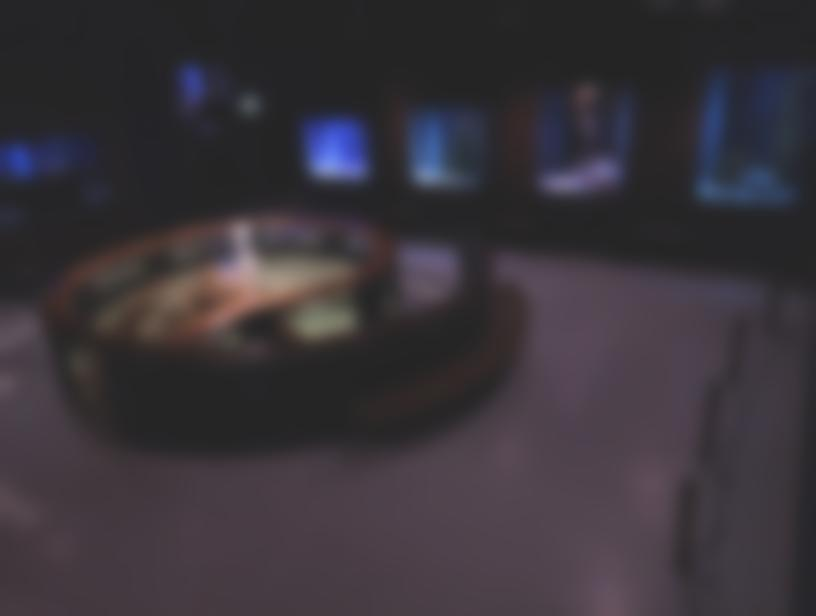
\includegraphics[width=\textwidth]{Images/DeviceImages/1st-iteration/hallvard-090224-141936-0-bright60.jpg}
        \caption{Brightness 60}
    \end{subfigure}
    \hfill
    \begin{subfigure}{0.30\textwidth}
        \centering
        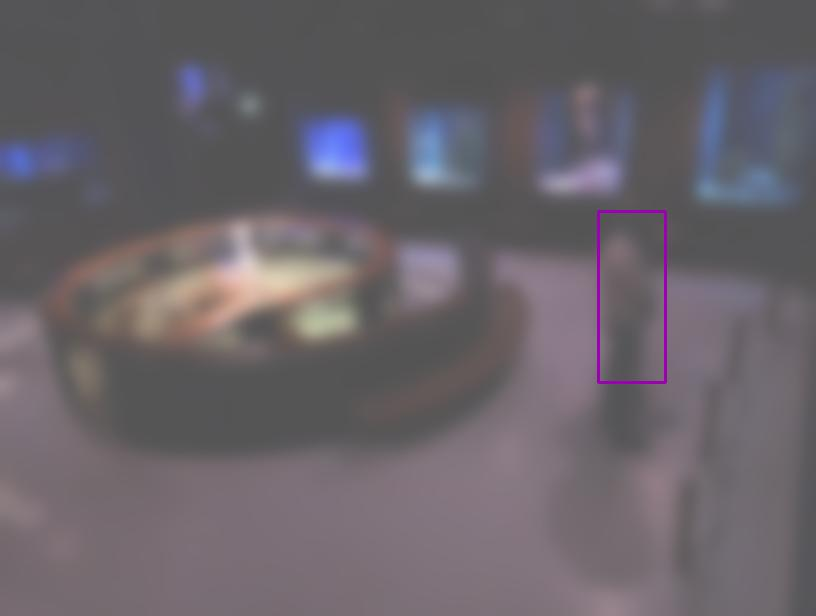
\includegraphics[width=1\textwidth]{Images/DeviceImages/1st-iteration/hallvard-090224-134417-1-bright70.jpg}
        \caption{Brightness 70}
    \end{subfigure}
    \hfill
    \begin{subfigure}{0.30\textwidth}
        \centering
        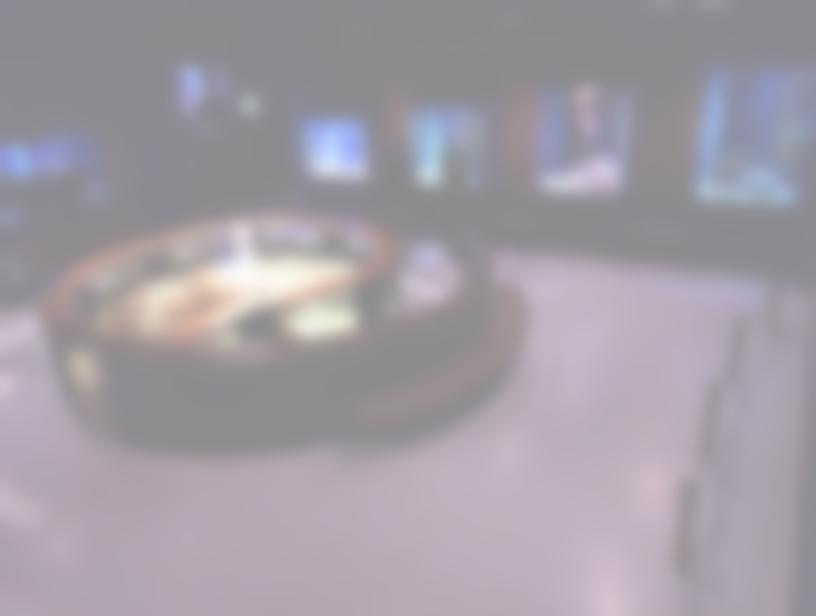
\includegraphics[width=\textwidth]{Images/DeviceImages/1st-iteration/hallvard-090224-132210-0-bright80.jpg}
        \caption{Brightness 80}
    \end{subfigure}
    \caption{Brightness values experimentation.}
    \label{fig:brightness_experimentation}
\end{figure}

Further, only one person is present in each image of the inconsistent partition of the dataset. This is to simulate the probable real-world scenario of having a single technician tasked with fine-tuning a detector. The inconsistent partition is suitable for testing how a poorly captured but highly relevant dataset may function as training data for model fine-tuning.

\paragraph{Consistent images}
The "Consistent-1" and "Consistent-2" partitions have consistent image characteritics. For these images, the camera settings were explicitly set to experimentally proven values to achieve the best image quality. The camera settings may be seen in table \ref{tab:picamera_settings}. The consistent partition of the dataset contains images with 1-4 persons in each image. The consistent images are split in two partitions to facilitate experiments using one partition as training data and the other for evaluation. This is suitable for testing how a well-captured dataset may function as training data for model fine-tuning. The settings used are found in table \ref{tab:picamera_settings}.

\begin{table}[H]
    \centering
    \renewcommand{\arraystretch}{1.5} % Increase vertical padding
    \setlength{\tabcolsep}{1em}
    \begin{tabular}{|l|c|}
        \hline
        \rowcolor{gray!25}
        \textbf{PI Camera Property} & \textbf{Value} \\ \hline
        $awb\_gains$                & (1.5, 1.5)     \\ \hline
        $awb\_mode$                 & off            \\ \hline
        \textit{brightness}         & 55             \\ \hline
        \textit{contrast}           & 0              \\ \hline
        $exposure_compensation$     & 0              \\ \hline
        $exposure\_mode$            & off            \\ \hline
        $exposure\_speed$           & 79989          \\ \hline
        \textit{framerate}          & 6              \\ \hline
        \textit{iso}                & 640            \\ \hline
        $sensor\_mode$              & 3              \\ \hline
        $shutter\_speed$            & 80000          \\ \hline
        \textit{resolution}         & 3264x2464      \\ \hline
    \end{tabular}
    \caption{\centering Camera settings for the image capturing of 2nd and 3rd iteration of image capturing.}
    {See appendix \ref{app:camera_settings_explanation} for a more detailed explanation of the camera settings.}
    \label{tab:picamera_settings}
\end{table}

\subsubsection{The Image Capturing Process}
Images were captured using a script that sequentially recorded data, storing each image directly onto a 32GB micro SD card installed in the device. This local storage approach was adopted to eliminate data transmission costs and potential security risks associated with transmitting sharp, identifiable images over the internet. The class \textit{Image} from the python package \textit{PIL} was used to store the images, and to address the limited storage capacity on the computer storing the dataset images, a save quality of 90 was used for all the images.

The dataset was built capturing images while no other visitors were present in the aquarium expect those who'd volunteer to participate. This was due to the restriction detailed in the project scope (section \ref{sec:scope_opening_hours}). A way to cancel image capturing was needed in case visitors entered the room. The simplest way of achieving this would be to pull the plug. This was challenging, however, as the devices and their power supplies were mounted high on the wall. The selected approach was to SSH\footnote{(Secure Shell (SSH) is not detailed in this thesis, see section \ref{sec:scope_ssh})} into the devices to start and stop the image capturing process.

Note that the ordering matters when setting the picamera properties. The ordering used to achieve consistent image capturing for project of this thesis is displayed in figure \ref{fig:code_camerahandler} in appendix \ref{app:code_snippets}.

Every once in a while, when a lot of visitors entered the room, the devices were demounted and the SD card plugged into the computer to extract the captured images. This resulted in slightly different angles when remounting the device, as finding the same configuration was challenging.

\paragraph{1st iteration: the inconsistent images}
\textit{Total number of images: 1312 (day 1), 986 (day 2) and 641 (day 3), total 2939. 1 subject.}

The first iteration of image capture was made with non-optimized camera configurations. To sufficiently brighten the images, the picamera.brightness attribute was set to 65. This is a postprocessing operation, which gave brighter but also artificially lit images. Also, the camera would sometimes focus on the bright fish-tanks in the museums, rendering the rest of the image rather dark. This was an effect of the awb mode and exposure mode being set to auto, and led to images of varying brightness and color. These images were still included in the dataset however, as images seen as suboptimal to the human eye may still be useful to the training of detectors. These images may be used to inspect the impact of captured image quality on inference performance.

The images were then used to build a proof of concept for the project pipeline, verifying and developing the steps needed for a successful project. The following steps in the project pipeline are described after the description of the 2nd and 3rd iterations of image captures.

Due to many technical difficulties the first few times images were being captured for the dataset, only the developer and author of this thesis is present in the images\footnote{Initially, an attempt was made to pass MQTT messages as a way to initialize image capture so multiple cameras could be deployed in several locations, thus speeding up and simplifying the image capturing process. This was discarded due to technical difficulties related to efficiently stopping the image capturing. For this single-deployment angle and area project, however, the approach with ssh-ing into the device worked fine.}.

\paragraph{2nd iteration: the consistent-1 images}
\textit{Total number of images: 295. 1-4 subjects.}

For the second image-capturing session, the camera configurations had been more thorougly tested to obtain more consistent images in terms of colors and brightness. This means using non-auto auto white balancing and exposure settings, and reducing the amount of post-processing brightness adjustment. Also, some friends were invited in this session. Due to a reduced post-processing brightness augmentation, the exposure speed had to be increased to get sufficient light in the images. This meant more unclear outlines of moving subjects in the frame. It also meant more time was spent capturing and storing each image. This increased from 1.3$\frac{s}{image}$ to 6.3$\frac{s}{image}$, which means the time available for image capturing was spent less productively than with the previous camera configuration. Depending on the impacts of image consistency on inference accuracy vs. amount of training data, capturing with a higher exposure speed and then post-processing the images to be brighter might be the better solution. Also, as pointed out by TODO insert mikkels master, augmenting the brightness might only slightly impact the model performance. This is because a model may see slight differences in pixel-level values invisible to humans, thus enabling it to still recognize the patterns of human outlines. A sufficiently bright image would still be required for the sake of model verification and ground truth obtainment (by human annotators).

The camera was repositioned three times during this iteration of image capturing. This is a drawback as it complicates the process of mapping the person positions in the images to real world locations in the acquarium. This is because the positions are represented as x,y values from the corner of the image, and for a person standing at exactly the same position in two images, the x,y-values will differ if the camera position has moved. Serving as a dataset for machine learning applications and not for analytics generation based on real world positions, this was not an issue.

\paragraph{NoIR camera}
During the 2nd iteration of image capturing, 60 images with a Raspberry Pi NoIR camera module version 2.1 were captured to determine its efficacy in enhancing human detection under low-light conditions. The "no" in NoIR signifies it's lack of an infrared filter. It was hypothized by the author that this meant the camera could then operate with a lower shutter speed, which showed promising results in initial tests. However, once deployed in the aquarium, this proved to be wrong. The NoIR camera is said to give the ability to look in the dark \textit{with infrared lightning}. Despite its potential, the noir camera was used as a regular camera module thereafter, capturing a different angle than the first device, for the remaining image capturing iterations. The 60 images were not used in the project, as the models trained on inconsistent data had already been trained.

\paragraph{3rd iteration: the consistent-2 images}
\textit{Total number of images: 466. 1-2 subjects.}

Similar to the 2nd iteration, but with 1-2 subjects instead of 1-4.

\subsubsection{Labeling}
\label{sec:labeling}

The detector requires precise ground truth positions of persons for training, validation, and testing. This data is obtained through a process known as image labeling or annotation.

To expedite the labeling process, the images were initially processed using a pre-trained YOLOv9 model on the COCO dataset, rather than manually labeling each image. Out of the 2939 images in the first-iteration dataset, the model prosuced 1863 detections that needed verification. This includes modifications, deletions, and additions to the annotations. The remaining 1076 images, which had no initial detections, required manual labeling from scratch.

Additionally, validation of the annotations uncovered specific errors: in 74 images, moving seaweed in one of the fish tanks was mistakenly identified as a human due to its human-like movement and shape. In some of the images (see figure \ref{fig:seaweed_man}), this 'seaweed-man' was presumably more likely to be a person than the human. In another instance, a person carrying a ladder was incorrectly recognized as one person carrying another.

\begin{figure}[H]
    \centering
    \begin{subfigure}{0.60\textwidth}
        \centering
        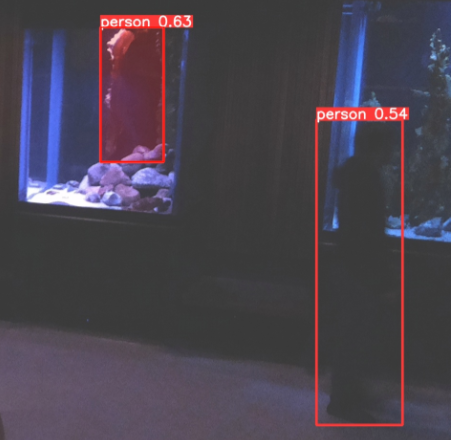
\includegraphics[width=\textwidth]{Images/Fun/seaweed-man-more-than-I.png}
        \caption{Seaweed and (presumably) a person}
    \end{subfigure}
    \hfill
    \begin{subfigure}{0.30\textwidth}
        \centering
        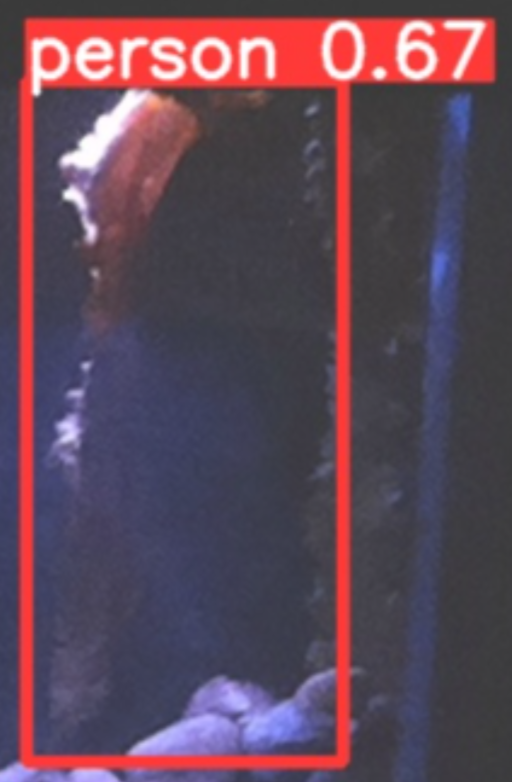
\includegraphics[width=\textwidth]{Images/Fun/seaweed-man-closeup.png}
        \caption{Seaweed-man}
    \end{subfigure}
    \caption{"Sometimes, it feels like the seaweed is more man than I" -Anonymous Visitor}
    \label{fig:seaweed_man}
\end{figure}

\paragraph{Label Studio}
"Label Studio" was used to label the images. This online tool allows for setting up a machine learning backend for automatically generating predictions for the images, to speed up the process. The setup of this backend was not trivial, however, and another approach was taken. The images were inferred on, the labels converted to label-studio json format, and then imported. This was a less 'automatic' approach but nevertheless effective. The label-studio tool was the used to modify, delete, and add annotations to the images. Finally, the annotations were exported and converted to the YOLO format. The code for converting yolo-to-label-studio and label-studio-to-yolo is found in Other/Code/Utils on \href{https://github.com/Hallvaeb/masterthesis}{https://github.com/Hallvaeb/masterthesis}.

\subsection{External Datasets}
This project utilizes multiple external datasets for developing and testing the object detection models. Each dataset was selected based on its relevance to the project, specifically for containing labeled images of the person class, and they vary in the number of images, capturing angle, and image diversity.

\subsubsection{Common Objects in Context (COCO)}
\label{sec:dataset_COCO}
The COCO dataset is a large dataset of 118 000 images and 80 different classes. The COCO-2017 train dataset was used to pre-train the models. The COCO-2017 validation dataset was used to evaluate the performance of the finalized models, as is industry standard. 

\subsubsection{CrowdHuman}
\label{sec:dataset_CrowdHuman}
CrowdHuman, the largest dataset used, focuses exclusively on images where people are the main subject, contrasting with COCO’s broader class range. This dataset was employed to assess how additional data might enhance model performance, with experiments conducted across various training data volumes.

\subsubsection{Person Reidentification in the Wild}
\label{sec:dataset_PRW}
Person Reidentification in the Wild comprises 11,816 images of pedestrians and aligns closely with our application needs as it exclusively contains images of people. This dataset's relevance is heightened by the presence of occlusions and the similar scale of persons to those detected in the aquarium setting. The dataset contains 932 individuals, annotated in 34 304 separate annotated boxes. Although designed to facilitate the development of reidentification applications, this functionality was not utilized in this project (refer to the project scope in section \ref{sec:scope_object_detection} for details). 

% \subsubsection{Football Players}
% The football-players dataset, characterized by its uniform perspective and consistent lighting and quality, was introduced to determine whether model improvements derive solely from specializing to single-class data or if the specialization's quality and relevance are crucial. It also provides a clear contrast in dataset characteristics, aiding in attributing performance differences to dataset nature rather than other confounding factors.


\subsection{Model Training}
\label{sec:model_training}


\paragraph{Licensing}
An effort has been made to keep the solution free and open to use, but some conditions may apply. The object detection algorithm YOLOv9 is under a GPL-3.0 License. This is a copy-left licensing, meaning it is free to use but has the requirement that any derivative works are released under the same rights. Another algorithm discussed in this thesis, the YOLOv3, is under a free-to-use license (AGPL-3.0), but changing the code is not allowed. The final object detector discussed, which could provide a solution for a company interested in keeping their solution hidden from competitors, is the DETR algorithm. This is under an Apache-2.0 license, which permits users to use and modify the code to fit their needs.

\subsubsection{Transfer Learning}
In this thesis, we are transferring the knowledge of a model that is pre-trained on a general dataset, to a model that is optimized for an aquarium environment. The general dataset in this case is the COCO dataset, a large dataset of 118 000 images and 80 different classes.

\subsubsection{Hyperparameter Tuning}
todo finskriv... Not really optimization.. More like finding... Since we're doing a cheeky approach to this. Done with autogluon, follow this guide for installation: \href{https://auto.gluon.ai/stable/install.html}{AutoGluon guide}. I had to run pip install autogluon twice for the imports to see autogluon.

\href{https://auto.gluon.ai/scoredebugweight/tutorials/course/script.html}{This guide} could be used to fine tune the hyperparameters of the model. A simpler guide was implemented to find the hyperparameters. This was to save time, and since our models require an okay level of hyperparameters. However, this choice to not give every dataset the same "fighting chance" with their optimal hyperparameters might have led to a lower validity of this experiments results.

Experiment 1: Do we need to run inference on the whole 2939 images to evaluate our model performance or will the results of evaluation on a subset be relative to the results of evaluation on the whole?

The standard yolov3 and yolov9 models were tested on the 1st and 2nd iteration images to see their out-of the box performance. Then, the yolov9 (which performed slightly better) was ran again but with a higher imgsz which typically increases the accuracy of the model. The three inferences: 1) yolov3 with imgsz 1280, 2) yolov9 with imgsz 1280 and 3) yolov9 with imgsz 1280 were then evaluated on the 1st iteration images and 2nd iteration images.

As expected, the inferences using a hightened imgsz was better. Another key takeaway was that the scores were relative, meaning evaluating on the full dataset was unnecessary. Moving forward, the 2nd iteration images from the acquarium were used to evaluate the models, while the 1st iteration images were used for training (and validation). This decision is also motivated by the fact that the 2nd iteration images are the most similar to the real-world application of the models.

We'd like the hyperparameter tuning process to focus on finding the hyperparameters that will best infer on images from the 2nd iteration. Therefore, an amateur would plan to tune the hyperparameters for each of the models using their respective dataset's training data and the 2nd iteration FIMUS dataset for validation data. This means the yolov9 CrowdHuman Smodel would use the same data for validation and testing, but only to find the right hyperparameters. Then, after using the testing data for tuning the hyperparameters, we replace the FIMUS 2nd iteration images for the datasets validation images and train the models using the optimal hyperparameters. This as a method to find the optimal hyperparameters may seem intuitive, as it has the strength of focusing on the right data when doing transfer learning with data other than the specialized task the model is specializing for. This means that the models would, during training, train to infer on data different from what it sees during training, which is what it will be doing after deployment.

The aforementioned approach is completely ignorant to how machine learning works, however. In supervision machine learning, the validation set is used to tune the hyperparameters, and the test set is used to evaluate the model's performance. The test set should be representative of the data the model will see after deployment, and the validation set should be representative of the data the model will see during training. The test set should not be used to tune the hyperparameters, as this would lead to overfitting the model to the test data.

Then, the . Tuning the hyperparameters for the test data means that the validation data used for training later will not at all be representative of the situation earlier, meaning the optimal hyperparameters will no longer be valid. Such an approach would not

What makes this project interesting is not the varying nature of datasets. Usually, one wants the best, most similar, and most data possible, and it's therefore irrelevant to see what using a less relevant dataset would do to the model. In this project the focus is more about how much of the high quality data is needed to make an impact. If 100 labeled images does the same work as 1000, then much work can be saved by only labeling 100 images. If only 100 images is needed then setting up a proper labeling tool might not even be necessary, as it may be done faster using a sub-optimal but fast-to-employ labeling tool. The insights may also be useful when

\subsection{Model Evaluation}


\subsection{Ethical Considerations}
In the deployment of advanced machine learning technologies for visitor localization and engagement analysis, this research proactively addresses privacy concerns through the implementation of image obscuration techniques. These methods ensure that no personally identifiable information is captured or communicated, thus significantly reducing privacy risks associated with visitor tracking in cultural spaces such as museums and aquariums.

\subsubsection{Privacy by Design}
At the forefront of our ethical approach is the principle of "privacy by design." This concept involves integrating privacy into the development and operation of our tracking technologies from the outset, rather than as an afterthought. By employing image obscuration techniques, such as real-time pixelation or silhouette generation, we ensure that the visual data processed by our system remains anonymous. This method effectively eliminates the possibility of identifying individual visitors from the captured data, thereby safeguarding their privacy.

The application of these privacy-preserving techniques negates the need for explicit consent from visitors for two primary reasons. First, the anonymization process occurs instantaneously as the data is captured, meaning no identifiable information is ever stored or analyzed. Second, the focus of the research is on aggregate behavior patterns rather than individual actions, further distancing the study from privacy concerns.

\subsubsection{Ethical Use and Data Protection}
Ensuring the ethical use of technology extends beyond privacy considerations to include the responsible handling and protection of any data generated by the system. Although the data is anonymized, we are committed to maintaining high standards of data protection. This includes secure data storage, limiting access to authorized personnel, and employing robust data management policies that comply with relevant data protection laws and guidelines.

The utilization of anonymization techniques also reflects our commitment to minimizing any potential impact on visitor behavior and the overall museum or aquarium experience. By ensuring that the tracking system is unobtrusive and does not compromise privacy, we aim to maintain the integrity of the visitor experience, allowing individuals to engage with exhibits without concern for their privacy.

\subsubsection{Transparency and Accountability}
While the technical approach effectively addresses privacy concerns, maintaining transparency about the use and purpose of tracking technologies is still essential. Information about the tracking system and its privacy-preserving nature will be made available to visitors, ensuring they are informed about how data is used to enhance the visitor experience.

Furthermore, the project will adhere to an ongoing ethical review process, ensuring that all aspects of the research remain aligned with ethical best practices and respond to evolving technological and societal standards.

In summary, by prioritizing privacy through the use of image obscuration techniques and adopting a comprehensive ethical framework, this research aims to advance the understanding of visitor engagement in a manner that is both innovative and respectful of individual privacy rights. This approach sets a precedent for the ethical application of machine learning technologies in cultural institutions, balancing the benefits of visitor behavior analysis with the imperative of protecting privacy.


\subsection{Heatmaps}
\label{sec:heatmaps}
Heatmaps are a powerful visualization tool that can provide insights into visitor behavior patterns and engagement levels within a museum or aquarium setting. By aggregating anonymized data from the tracking system, heatmaps can reveal areas of high visitor activity, peak visitation times, and popular exhibit locations. These visual representations offer valuable information for museum staff and curators, enabling them to optimize exhibit layouts, plan interactive experiences, and enhance visitor engagement. For this project, heatmaps were attempted to be created using 3 different python packages.

\paragraph{On the attempts to make heatmaps}
The first attempt was made asking chatGPT 4 to provide the code. The AI chose to draw circles using the python package "OpenCV", which without modifications did not render satisfactory results. Instead of tweaking a suboptimal solution, the attempt was then made to use the modules from Ultralytics to create the heatmap. The results of the first attempts may be seen in figure \ref{fig:heatmap_drafts}.

Ultralytics, a company from Los Angeles, is the same company that developed YOLOv5 on which the YOLOv9 is built upon. They also have premade modules for creating heatmaps. However, the solution neccessitates a detector model to make inferences live, and has no optional arguments to pass your own inferences. An attempt was made to modify the code and pass mock-data in the right format, but the result was unsatisfactory. The heatmaps were thus created with another module instead.

\begin{figure}[H]
    \centering
    \begin{subfigure}{0.45\textwidth}
        \centering
        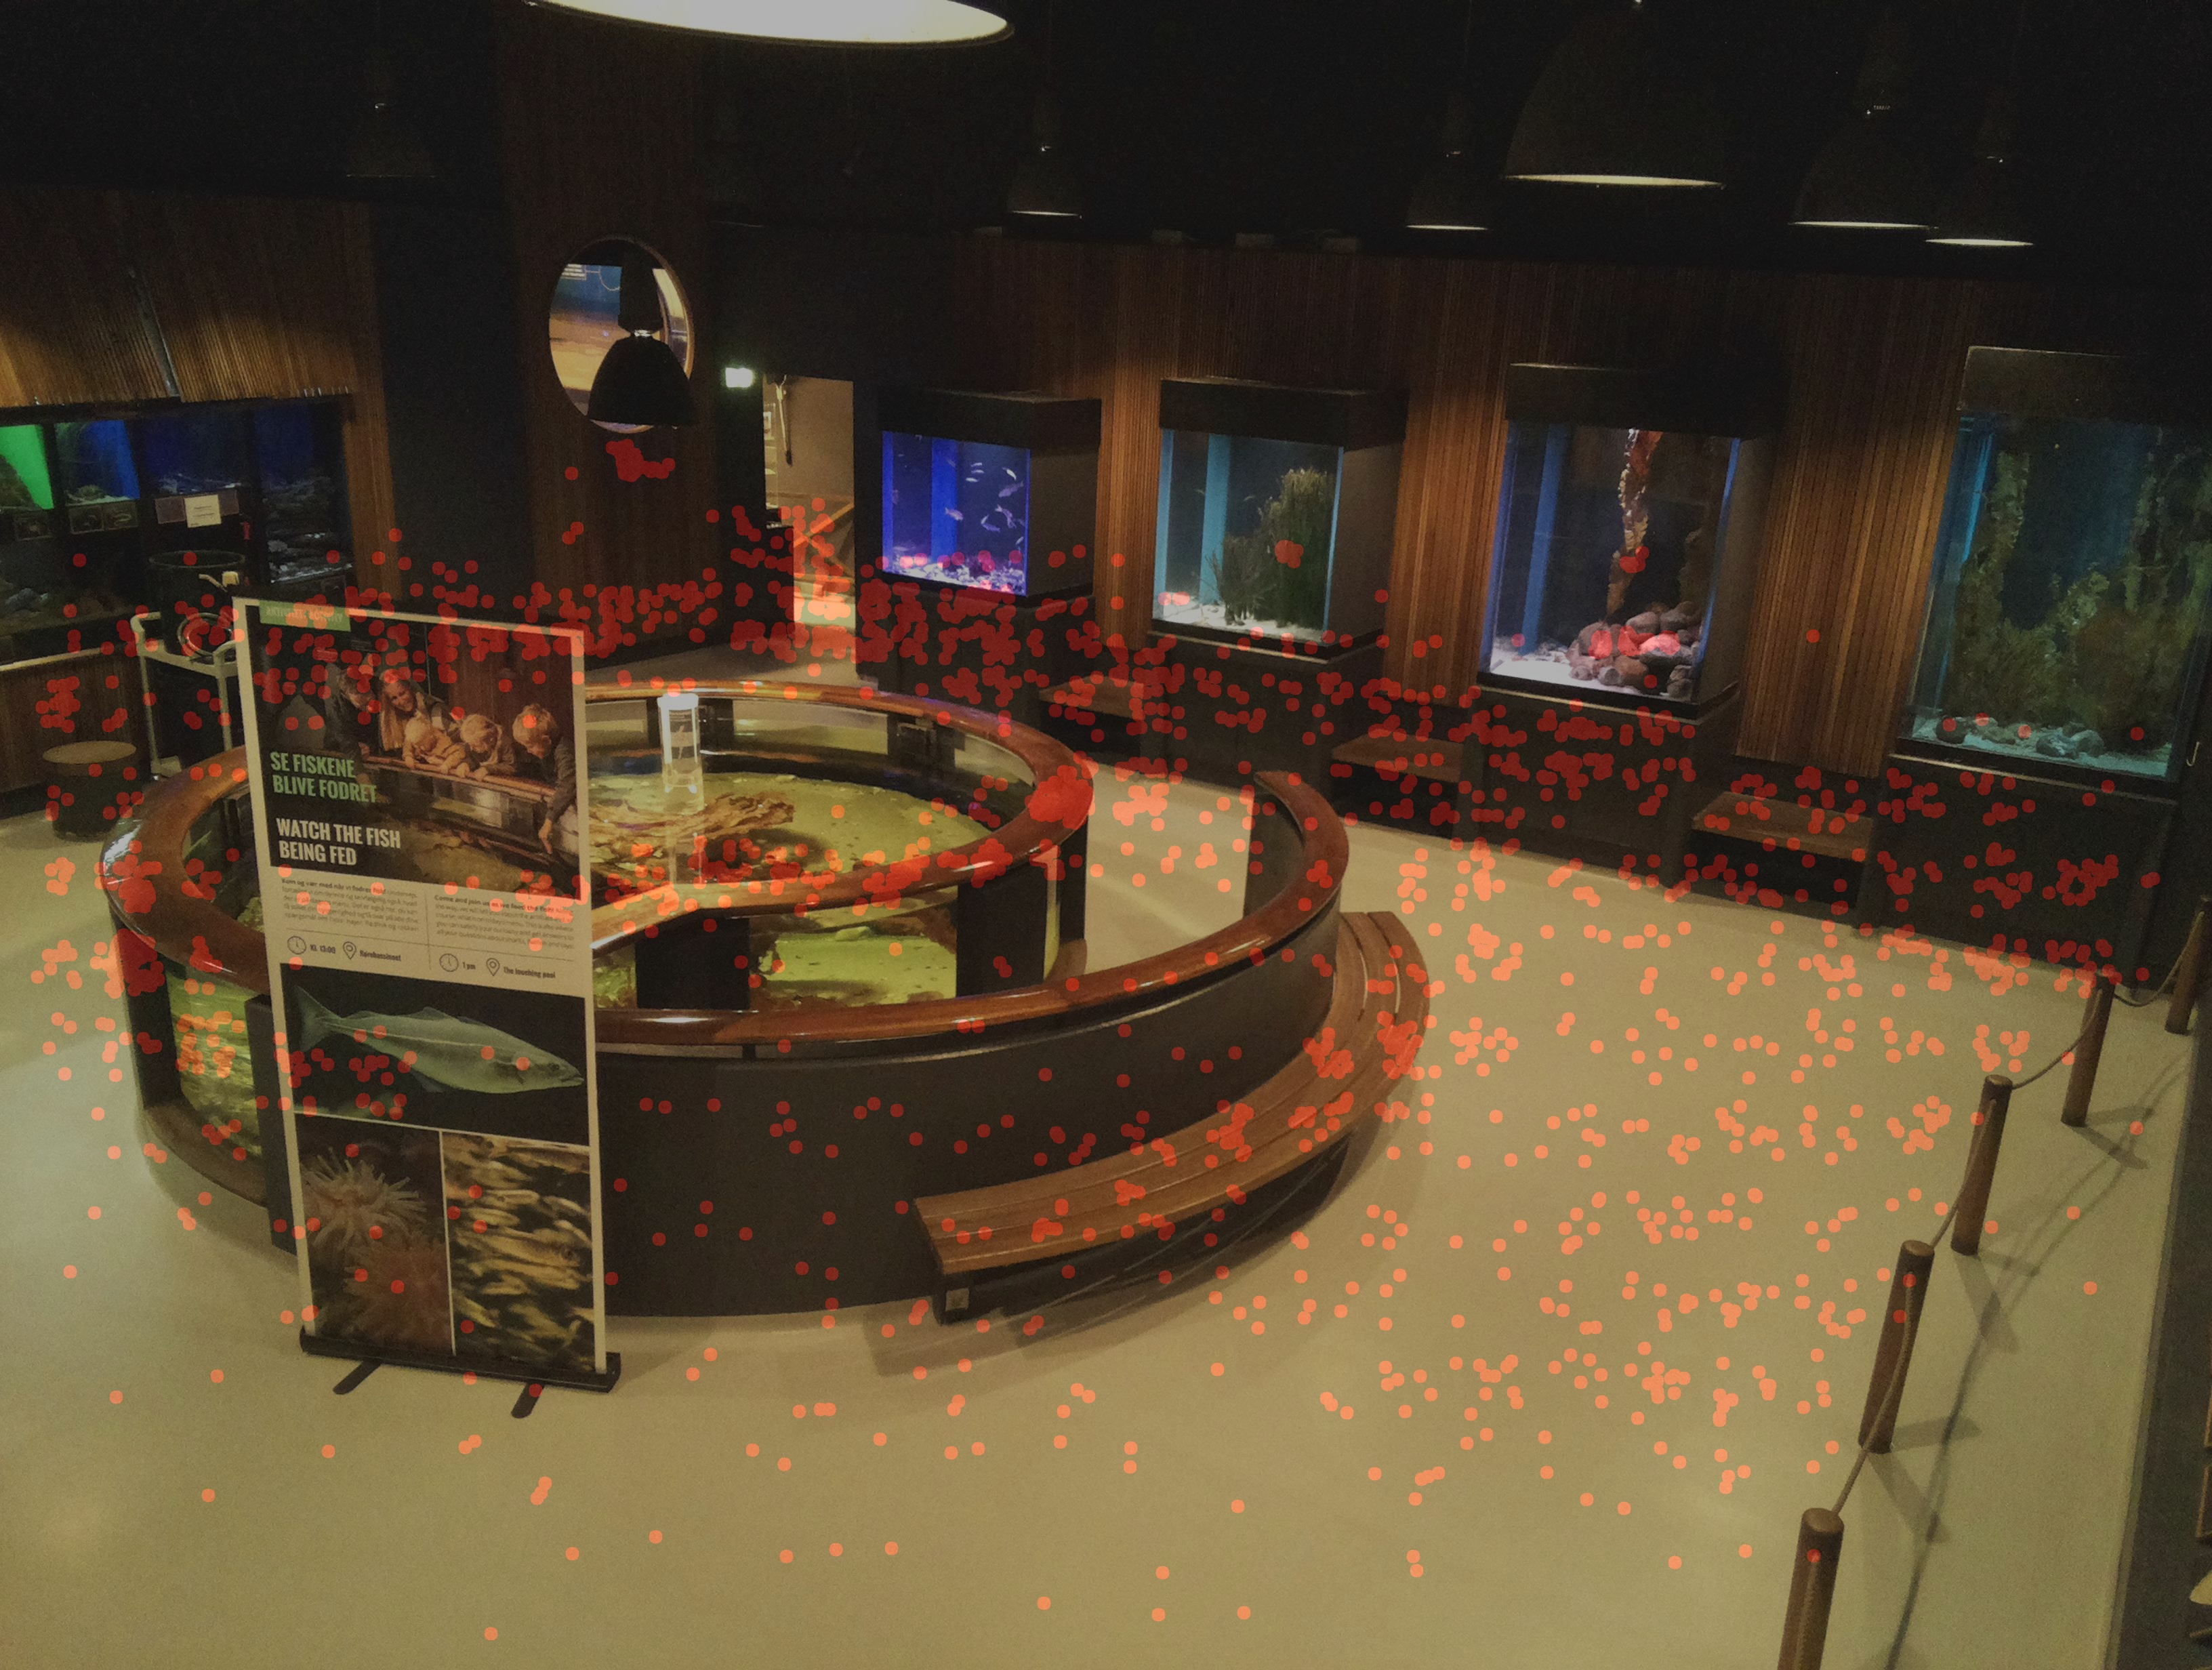
\includegraphics[width=\textwidth]{Images/Analytics/heatmap_gpt.jpg}
        \caption{Heatmap Draft 1: ChatGPT-4 solution}
    \end{subfigure}
    \hfill
    \begin{subfigure}{0.45\textwidth}
        \centering
        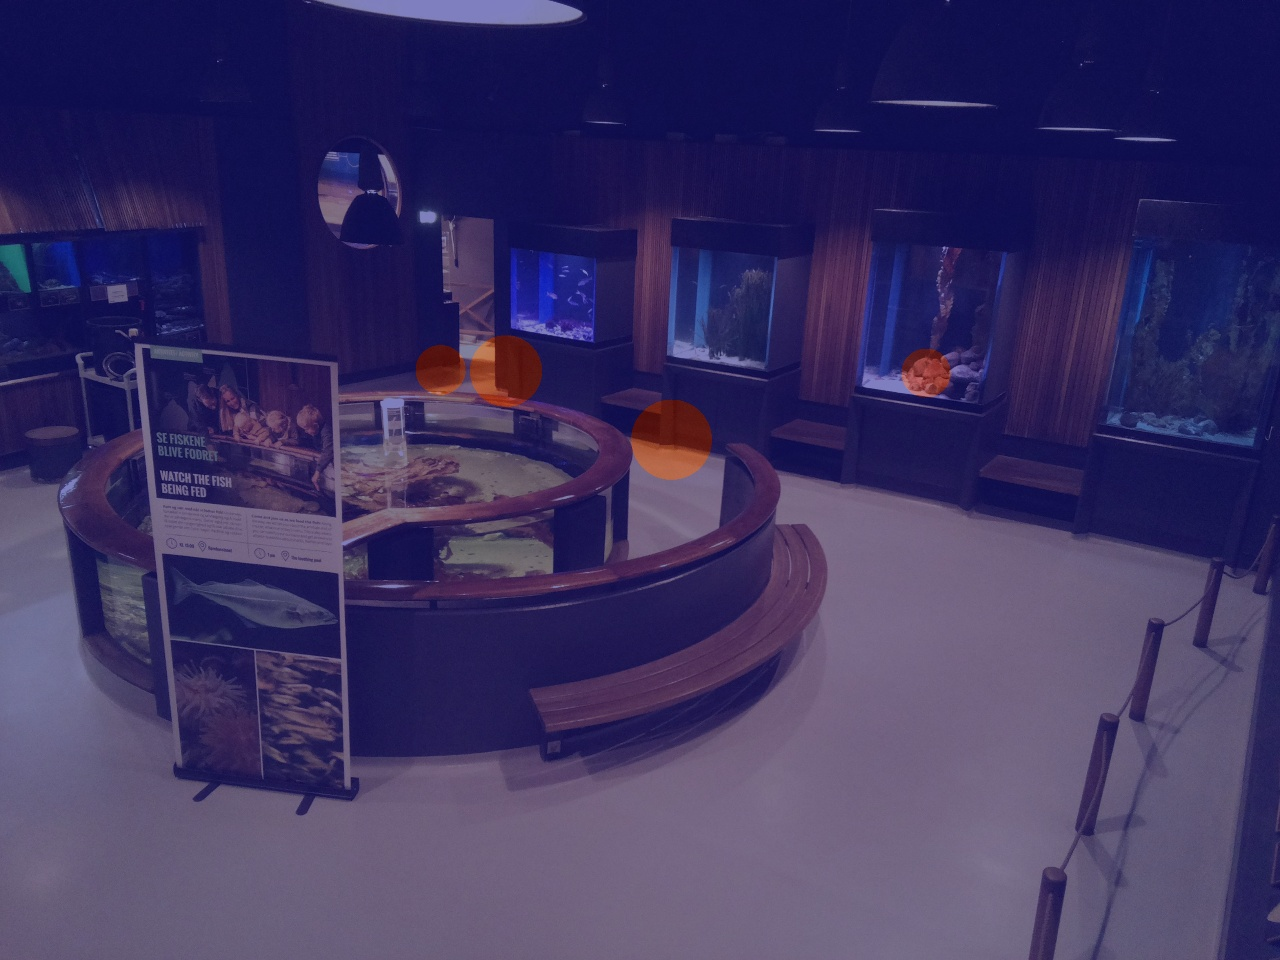
\includegraphics[width=1\textwidth]{Images/Analytics/heatmap_ultralytics.jpg}
        \caption{Heatmap Draft 2: Ultralytics solution}
    \end{subfigure}
    \caption{Heatmap Development Drafts}
    \label{fig:heatmap_drafts}
\end{figure}

\subsubsection{Supervision Heatmaps}
Supervision is a module created by Roboflow, to make reusable and user friendly computer vision tools. It is designed to be model agnostic. The github repo may be found \href{https://github.com/roboflow/supervision}{here}.

The solution incorporating Supervision rendered satisfactory results and may be seen in figure \ref{fig:heatmap_final}. This solution supports generating heatmaps from data in a pandas dataframe, allowing for filtering the dataframe to generate the preferred heatmaps based on for example the relevant times of the day or for the correct time interval.

\subsection*{Notes}

Tried to download/use model from Roboflow, but either image has to be sent to an API which would not retain privacy, or the device has to host an API itself to run the inference... Seems unlikely to be the most preferable solution, as the device would have to set up the service and run it locally. 

Possibly an interesting solution would be to do this with multiple devices. This supports the master-slave pattern of having multiple weaker computers and have them send to the stronger unit. 
Setting up private TCP connection between the weaker units and the strong unit and have the images sent to the stronger, so it can detect on them and send information etc. How many weak units do we need in order to make it profitable to have a strong GPU unit to do the processing? This whole systems sounds to be a complicating setuo process, not making the product modular and easy-to-use. Includes a lot of connection/networking to make the weaker units find and connect to strong, physically close device.

This task would mean setting up a strong device to host a network to which the weak units might connect to, and send images to. The issue is whenever images are sent, a lot of transmission is used... But the model takes image input size of 416x416. Would it be similar to just downscale the image before sending, or would this give the model less detail to work with?

Will now run several models on datasets from the web, i.e. the CrowdHuman dataset to see their accuracies. Will then deploy the models to device in acquarium to see if the best-performing model is an option in terms of size and inference speed. If it is preferable, I will attempt to increase it's accuracy by accumulating and annotating a specialized dataset for that setting, and training the final layers on the data. Can this be done with a



% A lot of time was spent setting up the arrangement in the acquarium and having the raspberry pi communicate correctly. The dataset collection process was also time-consuming, as it required the acquarium to be empty of non-consenting persons. Precautions were made in order not to upset the acquarium staff. This included not capturing outside opening hours, and not asking the visitors themselves if they could be in the images. The initial idea was to send a start-capture signal to the devices, and then a stop-capture signal once visitors entered the room. However, this was more time-consuming to set up than anticipated, as the choice was made to make them communicate over usb-mobile network connections.